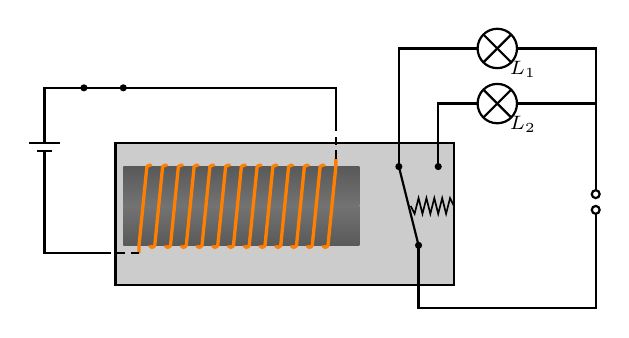
\begin{tikzpicture}
	% Kasten für Relais
	\draw [thick,fill=gray!40] (-0.1,-0.5) rectangle (4.2,1.3);
	%Eisenkern
	\shade [top color=gray!70!black, bottom color=gray!90!black] (0,0.5) rectangle (3,1);
	\shade [bottom color=gray!70!black, top color=gray!90!black] (0,0) rectangle (3,0.5);
	% Spule
	%Anfangspunkt (0.2,-0.1)
	\draw [color=orange, very thick] (0.2,-0.1) -- (0.2,0) -- ++(0.1,1) .. controls ++(0.05,0.04) and ++(0,0) .. ++(0.05,0);
	\foreach \x in {0.4,0.6,...,2.6} {
		\draw [color=orange, very thick] (\x-0.06,0) -- (\x-0.06,-0.01) .. controls ++(0.03,-0.04) and ++(0,0) .. (\x,0) -- ++(0.1,1) .. controls ++(0.05,0.04) and ++(0,0) .. ++(0.05,0);
	}
	\draw [color=orange, very thick] (2.6-0.06,0) -- (2.6-0.06,-0.01) .. controls ++(0.03,-0.04) and ++(0,0) .. (2.6,0) -- ++(0.1,1) -- ++(0,0.1);  % Endpunkt: (2.7,1.1)
	%%%% Steuerstromkreis
	\draw (2.7,1.1) [densely dashed, thick] -- (2.7,1.5);
	\draw [thick] (2.7,1.5) -- (2.7,2) -- (0,2);
	%Schalter geschlossen
	\draw [thick,fill=black] (0,2) circle [radius=0.03]; 
	\draw [thick] (-0.5,2) -- ++ (0.5,0);
	\draw [thick,fill=black] (-0.5,2) circle [radius=0.03]; 
	\draw [thick] (-0.5,2) -- (-1,2) -- (-1,1.3) ++(-0.2,0) -- ++(0.4,0) ++(-0.1,-0.1) -- ++(-0.2,0) ++(0.1,0) -- (-1,-0.1) -- (-0.2,-0.1);
	\draw [thick,densely dashed] (0.2,-0.1) -- (-0.2,-0.1);
	%%%% Arbeitsstromkreis
	%Wechselschalter
	\draw [thick, fill=black] (3.75,0) circle [radius=0.03];
	\draw [thick, fill=black] (3.5,1) circle [radius=0.03];
	\draw [thick, fill=black] (4,1) circle [radius=0.03];
	\draw [thick] (3.75,0) -- (3.5,1);
	%Feder
	\draw [semithick] (4.2,0.5) -- ++(-0.05,0.1) -- ++(-0.05,-0.2) -- ++(-0.05,0.2) -- ++(-0.05,-0.2) -- ++(-0.05,0.2) -- ++(-0.05,-0.2)-- ++(-0.05,0.2) -- ++(-0.05,-0.2)-- ++(-0.05,0.2) -- ++(-0.05,-0.2) -- ++(-0.05,0.1);
	% Stromkreis an sich
	\draw [thick] (3.75,0) -- (3.75,-0.8) -- (6,-0.8) -- (6,0.4);
	\draw [thick] (6,0.45) circle [radius=0.05];
	\draw [thick] (4,1) -- (4,1.8) -- (4.5,1.8);
	%Lampe L2
	\draw [thick] (4.75,1.8) circle [radius=0.25] node [below right =0.8] {\scriptsize $L_2$};
	\draw [thick] (4.75,1.8) -- ++(45:0.25);
	\draw [thick] (4.75,1.8) -- ++(135:0.25);
	\draw [thick] (4.75,1.8) -- ++(225:0.25);
	\draw [thick] (4.75,1.8) -- ++(315:0.25);
	%weiter mit Kabels
	\draw [thick] (5,1.8) -- (6,1.8) -- (6,0.7);
	\draw [thick] (6,0.65) circle [radius=0.05];
	\draw [thick] (3.5,1) -- (3.5,2.5) -- (4.5,2.5);
	%Lampe L1
	\draw [thick] (4.75,2.5) circle [radius=0.25] node [below right =0.8] {\scriptsize $L_1$};
	\draw [thick] (4.75,2.5) -- ++(45:0.25);
	\draw [thick] (4.75,2.5) -- ++(135:0.25);
	\draw [thick] (4.75,2.5) -- ++(225:0.25);
	\draw [thick] (4.75,2.5) -- ++(315:0.25);
	% Kabels
	\draw [thick] (5,2.5) -- (6,2.5) -- (6,1.8);
\end{tikzpicture}